\documentclass[twocolumn]{article}
\usepackage{subfig}
\usepackage{graphicx}
\begin{document}
	\title{\begin{titlepage}
			My paper
	\end{titlepage}}
	\section{1}
	\subsection{1.1}
	\subsection{1.2}
	\subsection{1.3}
	\subsection{1.4}
	
	\section{2}
	\subsection{2.1}
	\subsection{2.2}
	\subsection{2.3}
	\subsection{2.4}
	
	\section{3}
	\subsection{Thrust stand}
	%THE THRUST STAND
	In our setup we used a thrust stand obtained from RCBenchmark, specifically the RCBenchmark Thrust stand and Dynamometer Series 1580 \cite{rcb} as our testbed. The measurements from the thrust stand will be our "ground truth". This thrust stand incorporates a micro-controller board along with three, three-axis strain guage to measure the forces and the torque derived by the propeller. The board also collects data on the voltage, current and the signal to the ESC's which allows us to measure the power draw of the motor, and the RPM of the motor. Along with this there is an associated GUI which allows us to control the board and collect and visualize the data. The testbed collects data at a very high rate of close to 1kHz but then averages the data to eliminate outliers, so the data rate is 40Hz. This is more than adequate for the purposes of modeling the thrust response of the propeller to various stimuli. 
	\subsection{Wind Sensor Intro}
	The wind sensor we have chosen to use is the "Modern Device- Wind Sensor Rev. P" \cite{wind_sensor}. This device is a hot wire anemometer that is designed to measure wind from any direction. Hot wire anemometers work by passing a constant current through a thin wire which heats up due to the current. As the wind flows past the wire, the wire will be cooled down rapidly, resulting in a change in the measured voltage, which is the value that we observe \cite{hot_wire}. This system allows us to measure the wind speed that is resultant of the propeller. 
	\subsection{Wind Sensor Proof}
	To understand the limitations of the wind sensor, we performed a series of tests to characterize the sensor. The first of which was to determine under which orientation the sensor observed the highest range of wind speeds. As seen in \ref{orient_test}, the orientation of placing the wind sensor normal to the direction of wind flow allowed for the highest range of measurement. Next we performed a test to determine the feasible range of measurement. This was done by exposing the wind sensor to a step-signal test and a pulse signal test ranging from the minimal PWM value to approximately $50\%$ of the motor's max value, the results of which are in \ref{min_max}. The PWM values in this case are based around the Simulink-Arduino Library PWM module.  This resulted in a working range from $PWM = 44$ to $PWM = 60$. While there is possibility for the wind sensor to measure higher wind speeds, there is a significant amount of noise even with the addition of a low-pass filter, hence we decided to limit the max speed of our experiment. 
	
	Another factor that we deem is important to characterize is the speed of response to change of wind speed. We measured this by running the propeller at various different speeds, while tracking the thrust output on the testbed as our base measurement of response time and then comparing the response time to see the lag in response time. By doing this we found that there was a negligible lag time of less than $10 ms$, which is our resolution for each measurement.
	 
	Lastly we measured the location of the wind sensor in relation to the propellers. To do so we measured a semi-circle area behind the propeller to deem the location of highest wind sensitivity. Resulting in a map as seen in figure \ref{area}. 
	
	By characterizing the wind sensor, we can ensure that it is in the optimal configuration for us to collect data.
	
	\section{Results}
	
	\subsection{Experimental Setup- How we set up the kalman/Algorithm}
	\begin{figure}[b]
		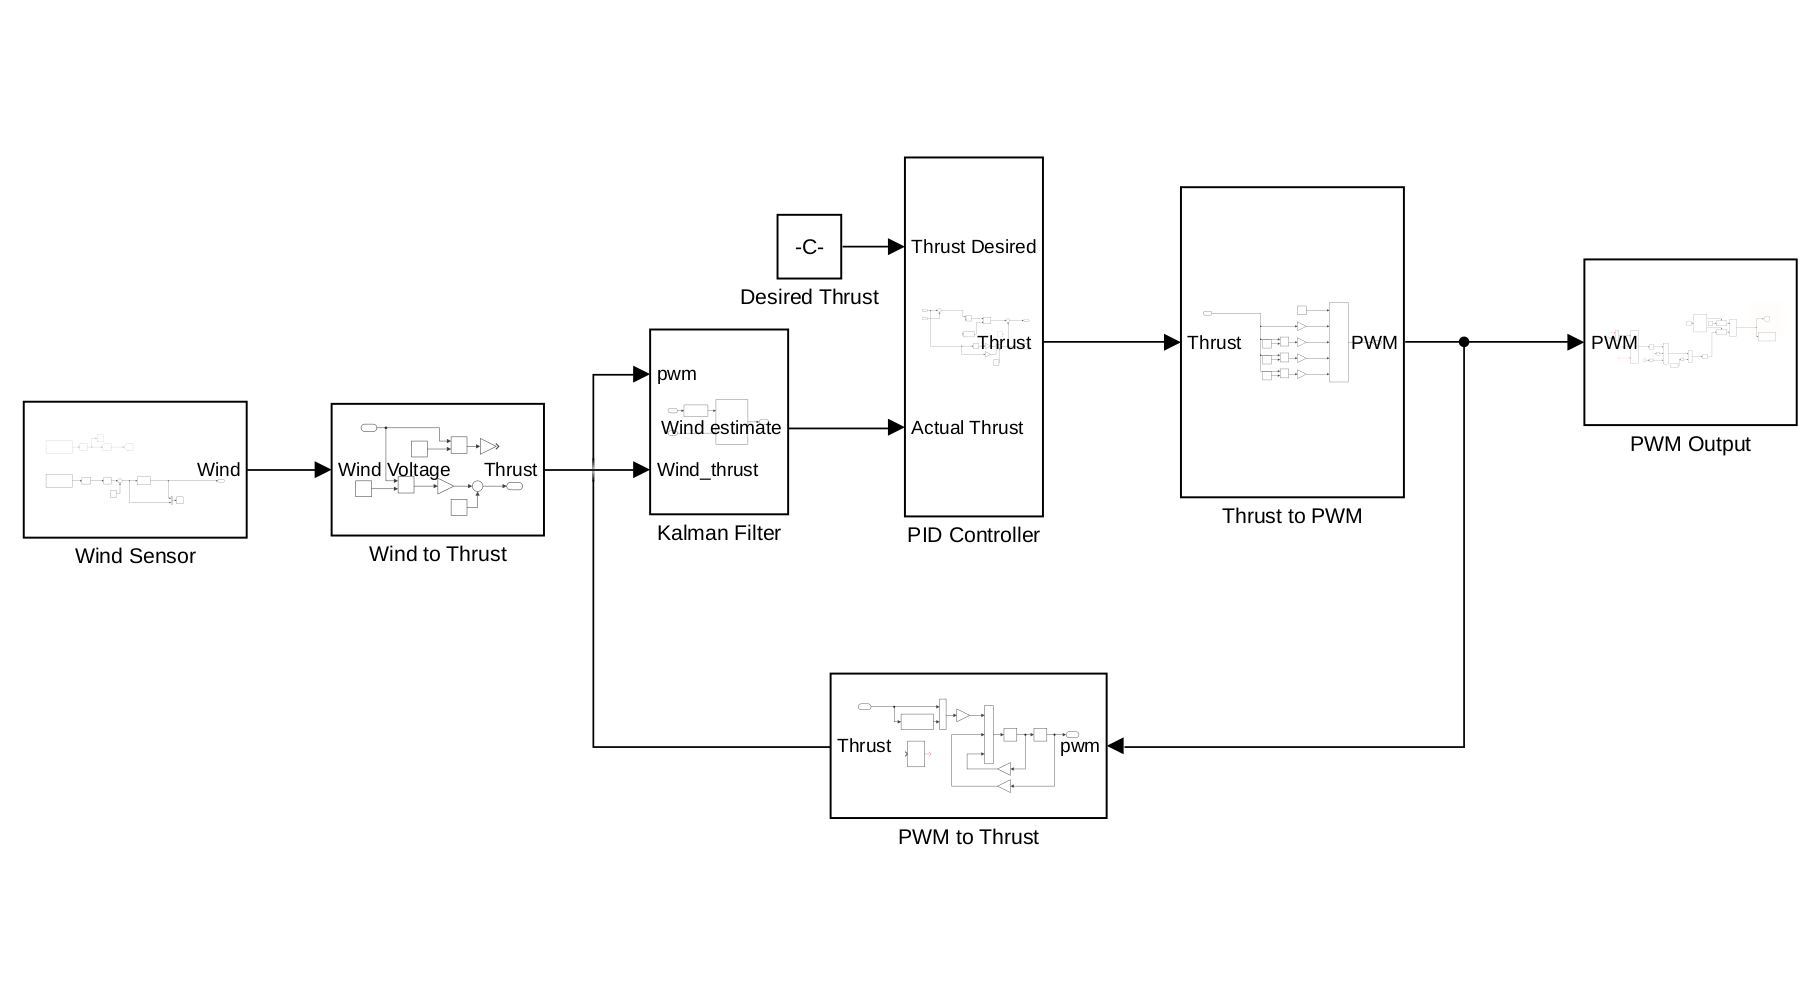
\includegraphics[width=\textwidth]{block_diagram}
		\caption{Block Diagram}
		\label{block_diagram}
	\end{figure}

	We developed a control architecture as pictured in fig \ref{block_diagram} where there are two sources of measurement for the thrust value. The first, main value, is from the wind sensor which is measured through an Arduino. The voltage value that the arduino measures is then converted to a thrust value through the power function
	\begin{equation}
	Thrust = 4.701 * 10^{15} * V_w^{6.146} + 0.0731
	\label{wind_power}
	\end{equation}
	
	The second measurement of thrust is a polynomial function that converts the recorded PWM value that is used to control the propeller to thrust. \newline
	\begin{eqnarray}
	Thrust = 1.957*10^{-5}*PWM^4 \\
	- 7.476*10^{-4}*PWM^3 \nonumber\\ 
	+ 1.272*10^{-2}*PWM^2 \nonumber\\
	+ .01092*PWM - .01842 \nonumber
	\label{pwm_poly}
	\end{eqnarray}
	
	These values are then passed through a Kalman Filter weighted for the wind sensor. This method allows for the system to accurately determine the thrust value output while reducing noise due to the nature of the wind. Next this value is passed to a PID controller which checks the current thrust value to the desired thrust value and outputs a thrust value. Lastly a polynomial function converts the thrust value back to PWM.
	\begin{eqnarray}
	PWM = -.1746*Thrust^4 + 1.008*Thrust^3\\ 
	- 3.409*Thrust*2 + 12.29*Thrust + 1.8430 \nonumber
	\label{pwm_poly}
	\end{eqnarray}
	\subsection{The tests}
	Once the characteristics of the wind sensor were determined we ran tests to ensure the viability of our algorithm and if it would respond to external stimuli the way we expected.
	\subsection{4.3}
	\subsection{4.4}
	
	\section{5}

	\subsection{5.1}
	\subsection{5.2}
	\subsection{5.3}
	\subsection{5.4}

	
	

	\begin{thebibliography}{99}
		\bibitem{Mahoney1} Mahoney 2012
		\bibitem{rcb} https://www.rcbenchmark.com/dynamometer-series-1580/
		\bibitem{wind_sensor} https://moderndevice.com/product/wind-sensor-rev-p/
		\bibitem{hot_wire} Extended Applications of the Hot‐Wire Anemometer, Stanley Corrsin,Review of Scientific Instruments 1947 18:7, 469-471 
		
	\end{thebibliography}


\end{document}